% Created by tikzDevice version 0.11 on 2018-03-29 18:14:07
% !TEX encoding = UTF-8 Unicode
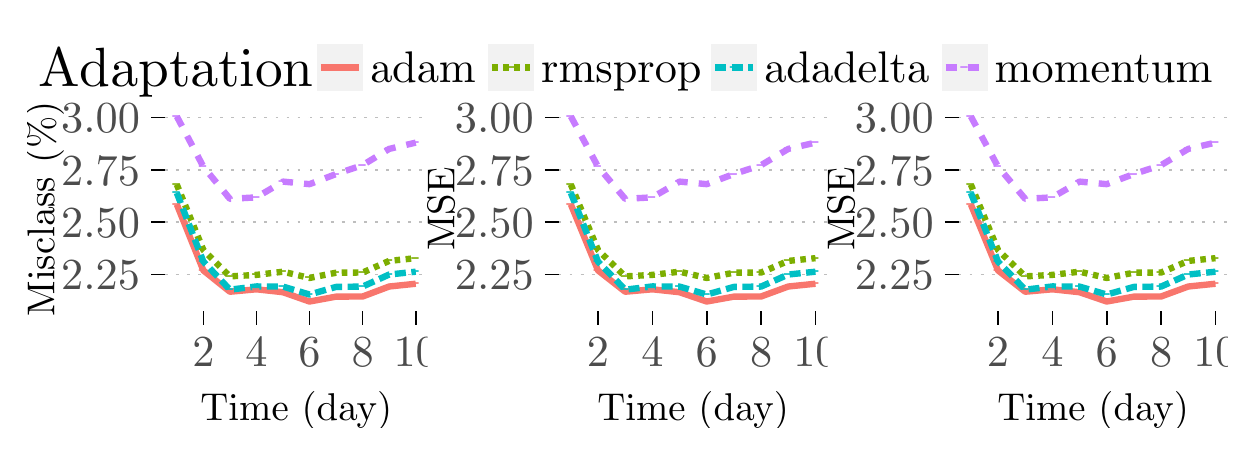
\begin{tikzpicture}[x=1pt,y=1pt]
\definecolor{fillColor}{RGB}{255,255,255}
\path[use as bounding box,fill=fillColor,fill opacity=0.00] (0,0) rectangle (433.62,144.54);
\begin{scope}
\path[clip] (  0.00,  0.00) rectangle (433.62,144.54);
\definecolor{fillColor}{RGB}{255,255,255}

\path[fill=fillColor] ( -1.83,115.81) rectangle (435.45,144.54);
\end{scope}
\begin{scope}
\path[clip] (  0.00,  0.00) rectangle (433.62,144.54);
\definecolor{drawColor}{RGB}{0,0,0}

\node[text=drawColor,anchor=base west,inner sep=0pt, outer sep=0pt, scale=  2.00] at (  3.86,123.29) {Adaptation};
\end{scope}
\begin{scope}
\path[clip] (  0.00,  0.00) rectangle (433.62,144.54);
\definecolor{drawColor}{RGB}{255,255,255}
\definecolor{fillColor}{gray}{0.95}

\path[draw=drawColor,line width= 0.6pt,line join=round,line cap=round,fill=fillColor] (104.19,121.50) rectangle (121.53,138.85);
\end{scope}
\begin{scope}
\path[clip] (  0.00,  0.00) rectangle (433.62,144.54);
\definecolor{drawColor}{RGB}{248,118,109}

\path[draw=drawColor,line width= 2.3pt,line join=round] (105.92,130.18) -- (119.80,130.18);
\end{scope}
\begin{scope}
\path[clip] (  0.00,  0.00) rectangle (433.62,144.54);
\definecolor{drawColor}{RGB}{248,118,109}

\node[text=drawColor,anchor=base,inner sep=0pt, outer sep=0pt, scale=  1.00] at (112.86,128.01) {-};
\end{scope}
\begin{scope}
\path[clip] (  0.00,  0.00) rectangle (433.62,144.54);
\definecolor{drawColor}{RGB}{255,255,255}
\definecolor{fillColor}{gray}{0.95}

\path[draw=drawColor,line width= 0.6pt,line join=round,line cap=round,fill=fillColor] (166.04,121.50) rectangle (183.39,138.85);
\end{scope}
\begin{scope}
\path[clip] (  0.00,  0.00) rectangle (433.62,144.54);
\definecolor{drawColor}{RGB}{124,174,0}

\path[draw=drawColor,line width= 2.3pt,dash pattern=on 2pt off 2pt ,line join=round] (167.78,130.18) -- (181.65,130.18);
\end{scope}
\begin{scope}
\path[clip] (  0.00,  0.00) rectangle (433.62,144.54);
\definecolor{drawColor}{RGB}{124,174,0}

\node[text=drawColor,anchor=base,inner sep=0pt, outer sep=0pt, scale=  1.00] at (174.71,128.01) {-};
\end{scope}
\begin{scope}
\path[clip] (  0.00,  0.00) rectangle (433.62,144.54);
\definecolor{drawColor}{RGB}{255,255,255}
\definecolor{fillColor}{gray}{0.95}

\path[draw=drawColor,line width= 0.6pt,line join=round,line cap=round,fill=fillColor] (246.62,121.50) rectangle (263.97,138.85);
\end{scope}
\begin{scope}
\path[clip] (  0.00,  0.00) rectangle (433.62,144.54);
\definecolor{drawColor}{RGB}{0,191,196}

\path[draw=drawColor,line width= 2.3pt,dash pattern=on 4pt off 2pt ,line join=round] (248.36,130.18) -- (262.23,130.18);
\end{scope}
\begin{scope}
\path[clip] (  0.00,  0.00) rectangle (433.62,144.54);
\definecolor{drawColor}{RGB}{0,191,196}

\node[text=drawColor,anchor=base,inner sep=0pt, outer sep=0pt, scale=  1.00] at (255.30,128.01) {-};
\end{scope}
\begin{scope}
\path[clip] (  0.00,  0.00) rectangle (433.62,144.54);
\definecolor{drawColor}{RGB}{255,255,255}
\definecolor{fillColor}{gray}{0.95}

\path[draw=drawColor,line width= 0.6pt,line join=round,line cap=round,fill=fillColor] (329.93,121.50) rectangle (347.27,138.85);
\end{scope}
\begin{scope}
\path[clip] (  0.00,  0.00) rectangle (433.62,144.54);
\definecolor{drawColor}{RGB}{199,124,255}

\path[draw=drawColor,line width= 2.3pt,dash pattern=on 4pt off 4pt ,line join=round] (331.66,130.18) -- (345.54,130.18);
\end{scope}
\begin{scope}
\path[clip] (  0.00,  0.00) rectangle (433.62,144.54);
\definecolor{drawColor}{RGB}{199,124,255}

\node[text=drawColor,anchor=base,inner sep=0pt, outer sep=0pt, scale=  1.00] at (338.60,128.01) {-};
\end{scope}
\begin{scope}
\path[clip] (  0.00,  0.00) rectangle (433.62,144.54);
\definecolor{drawColor}{RGB}{0,0,0}

\node[text=drawColor,anchor=base west,inner sep=0pt, outer sep=0pt, scale=  1.60] at (123.70,124.67) {adam};
\end{scope}
\begin{scope}
\path[clip] (  0.00,  0.00) rectangle (433.62,144.54);
\definecolor{drawColor}{RGB}{0,0,0}

\node[text=drawColor,anchor=base west,inner sep=0pt, outer sep=0pt, scale=  1.60] at (185.56,124.67) {rmsprop};
\end{scope}
\begin{scope}
\path[clip] (  0.00,  0.00) rectangle (433.62,144.54);
\definecolor{drawColor}{RGB}{0,0,0}

\node[text=drawColor,anchor=base west,inner sep=0pt, outer sep=0pt, scale=  1.60] at (266.14,124.67) {adadelta};
\end{scope}
\begin{scope}
\path[clip] (  0.00,  0.00) rectangle (433.62,144.54);
\definecolor{drawColor}{RGB}{0,0,0}

\node[text=drawColor,anchor=base west,inner sep=0pt, outer sep=0pt, scale=  1.60] at (349.44,124.67) {momentum};
\end{scope}
\begin{scope}
\path[clip] (  0.00,  0.00) rectangle (144.54,115.81);
\definecolor{drawColor}{RGB}{255,255,255}
\definecolor{fillColor}{RGB}{255,255,255}

\path[draw=drawColor,line width= 0.6pt,line join=round,line cap=round,fill=fillColor] (  0.00,  0.00) rectangle (144.54,115.81);
\end{scope}
\begin{scope}
\path[clip] ( 49.57, 42.24) rectangle (144.54,115.81);
\definecolor{fillColor}{RGB}{255,255,255}

\path[fill=fillColor] ( 49.57, 42.24) rectangle (144.54,115.81);
\definecolor{drawColor}{RGB}{255,255,255}

\path[draw=drawColor,line width= 0.3pt,line join=round] ( 49.57, 45.84) --
	(144.54, 45.84);

\path[draw=drawColor,line width= 0.3pt,line join=round] ( 49.57, 64.77) --
	(144.54, 64.77);

\path[draw=drawColor,line width= 0.3pt,line join=round] ( 49.57, 83.70) --
	(144.54, 83.70);

\path[draw=drawColor,line width= 0.3pt,line join=round] ( 49.57,102.63) --
	(144.54,102.63);

\path[draw=drawColor,line width= 0.3pt,line join=round] ( 53.89, 42.24) --
	( 53.89,115.81);

\path[draw=drawColor,line width= 0.3pt,line join=round] ( 73.07, 42.24) --
	( 73.07,115.81);

\path[draw=drawColor,line width= 0.3pt,line join=round] ( 92.26, 42.24) --
	( 92.26,115.81);

\path[draw=drawColor,line width= 0.3pt,line join=round] (111.45, 42.24) --
	(111.45,115.81);

\path[draw=drawColor,line width= 0.3pt,line join=round] (130.63, 42.24) --
	(130.63,115.81);
\definecolor{drawColor}{RGB}{190,190,190}

\path[draw=drawColor,line width= 0.6pt,dash pattern=on 1pt off 3pt ,line join=round] ( 49.57, 55.30) --
	(144.54, 55.30);

\path[draw=drawColor,line width= 0.6pt,dash pattern=on 1pt off 3pt ,line join=round] ( 49.57, 74.23) --
	(144.54, 74.23);

\path[draw=drawColor,line width= 0.6pt,dash pattern=on 1pt off 3pt ,line join=round] ( 49.57, 93.16) --
	(144.54, 93.16);

\path[draw=drawColor,line width= 0.6pt,dash pattern=on 1pt off 3pt ,line join=round] ( 49.57,112.09) --
	(144.54,112.09);
\definecolor{drawColor}{RGB}{255,255,255}

\path[draw=drawColor,line width= 0.6pt,line join=round] ( 63.48, 42.24) --
	( 63.48,115.81);

\path[draw=drawColor,line width= 0.6pt,line join=round] ( 82.67, 42.24) --
	( 82.67,115.81);

\path[draw=drawColor,line width= 0.6pt,line join=round] (101.85, 42.24) --
	(101.85,115.81);

\path[draw=drawColor,line width= 0.6pt,line join=round] (121.04, 42.24) --
	(121.04,115.81);

\path[draw=drawColor,line width= 0.6pt,line join=round] (140.22, 42.24) --
	(140.22,115.81);
\definecolor{drawColor}{RGB}{248,118,109}

\path[draw=drawColor,line width= 2.3pt,line join=round] ( 53.89, 80.67) --
	( 63.48, 56.82) --
	( 73.07, 49.12) --
	( 82.67, 50.00) --
	( 92.26, 48.94) --
	(101.85, 45.58) --
	(111.45, 47.35) --
	(121.04, 47.40) --
	(130.63, 51.01) --
	(140.22, 52.01);
\definecolor{drawColor}{RGB}{124,174,0}

\path[draw=drawColor,line width= 2.3pt,dash pattern=on 2pt off 2pt ,line join=round] ( 53.89, 87.86) --
	( 63.48, 64.20) --
	( 73.07, 54.67) --
	( 82.67, 55.21) --
	( 92.26, 56.36) --
	(101.85, 54.10) --
	(111.45, 56.00) --
	(121.04, 56.06) --
	(130.63, 60.26) --
	(140.22, 61.25);
\definecolor{drawColor}{RGB}{0,191,196}

\path[draw=drawColor,line width= 2.3pt,dash pattern=on 4pt off 2pt ,line join=round] ( 53.89, 84.83) --
	( 63.48, 60.03) --
	( 73.07, 49.87) --
	( 82.67, 51.04) --
	( 92.26, 50.98) --
	(101.85, 48.11) --
	(111.45, 50.87) --
	(121.04, 50.99) --
	(130.63, 55.34) --
	(140.22, 56.36);
\definecolor{drawColor}{RGB}{199,124,255}

\path[draw=drawColor,line width= 2.3pt,dash pattern=on 4pt off 4pt ,line join=round] ( 53.89,112.47) --
	( 63.48, 94.30) --
	( 73.07, 82.69) --
	( 82.67, 83.22) --
	( 92.26, 88.92) --
	(101.85, 87.99) --
	(111.45, 91.65) --
	(121.04, 94.86) --
	(130.63,100.73) --
	(140.22,103.00);
\definecolor{drawColor}{RGB}{248,118,109}

\node[text=drawColor,anchor=base,inner sep=0pt, outer sep=0pt, scale=  1.00] at ( 53.89, 78.50) {-};

\node[text=drawColor,anchor=base,inner sep=0pt, outer sep=0pt, scale=  1.00] at ( 63.48, 54.65) {-};

\node[text=drawColor,anchor=base,inner sep=0pt, outer sep=0pt, scale=  1.00] at ( 73.07, 46.95) {-};

\node[text=drawColor,anchor=base,inner sep=0pt, outer sep=0pt, scale=  1.00] at ( 82.67, 47.84) {-};

\node[text=drawColor,anchor=base,inner sep=0pt, outer sep=0pt, scale=  1.00] at ( 92.26, 46.78) {-};

\node[text=drawColor,anchor=base,inner sep=0pt, outer sep=0pt, scale=  1.00] at (101.85, 43.42) {-};

\node[text=drawColor,anchor=base,inner sep=0pt, outer sep=0pt, scale=  1.00] at (111.45, 45.19) {-};

\node[text=drawColor,anchor=base,inner sep=0pt, outer sep=0pt, scale=  1.00] at (121.04, 45.23) {-};

\node[text=drawColor,anchor=base,inner sep=0pt, outer sep=0pt, scale=  1.00] at (130.63, 48.85) {-};

\node[text=drawColor,anchor=base,inner sep=0pt, outer sep=0pt, scale=  1.00] at (140.22, 49.84) {-};
\definecolor{drawColor}{RGB}{124,174,0}

\node[text=drawColor,anchor=base,inner sep=0pt, outer sep=0pt, scale=  1.00] at ( 53.89, 85.70) {-};

\node[text=drawColor,anchor=base,inner sep=0pt, outer sep=0pt, scale=  1.00] at ( 63.48, 62.04) {-};

\node[text=drawColor,anchor=base,inner sep=0pt, outer sep=0pt, scale=  1.00] at ( 73.07, 52.51) {-};

\node[text=drawColor,anchor=base,inner sep=0pt, outer sep=0pt, scale=  1.00] at ( 82.67, 53.04) {-};

\node[text=drawColor,anchor=base,inner sep=0pt, outer sep=0pt, scale=  1.00] at ( 92.26, 54.20) {-};

\node[text=drawColor,anchor=base,inner sep=0pt, outer sep=0pt, scale=  1.00] at (101.85, 51.94) {-};

\node[text=drawColor,anchor=base,inner sep=0pt, outer sep=0pt, scale=  1.00] at (111.45, 53.84) {-};

\node[text=drawColor,anchor=base,inner sep=0pt, outer sep=0pt, scale=  1.00] at (121.04, 53.90) {-};

\node[text=drawColor,anchor=base,inner sep=0pt, outer sep=0pt, scale=  1.00] at (130.63, 58.10) {-};

\node[text=drawColor,anchor=base,inner sep=0pt, outer sep=0pt, scale=  1.00] at (140.22, 59.08) {-};
\definecolor{drawColor}{RGB}{0,191,196}

\node[text=drawColor,anchor=base,inner sep=0pt, outer sep=0pt, scale=  1.00] at ( 53.89, 82.67) {-};

\node[text=drawColor,anchor=base,inner sep=0pt, outer sep=0pt, scale=  1.00] at ( 63.48, 57.87) {-};

\node[text=drawColor,anchor=base,inner sep=0pt, outer sep=0pt, scale=  1.00] at ( 73.07, 47.71) {-};

\node[text=drawColor,anchor=base,inner sep=0pt, outer sep=0pt, scale=  1.00] at ( 82.67, 48.88) {-};

\node[text=drawColor,anchor=base,inner sep=0pt, outer sep=0pt, scale=  1.00] at ( 92.26, 48.82) {-};

\node[text=drawColor,anchor=base,inner sep=0pt, outer sep=0pt, scale=  1.00] at (101.85, 45.94) {-};

\node[text=drawColor,anchor=base,inner sep=0pt, outer sep=0pt, scale=  1.00] at (111.45, 48.70) {-};

\node[text=drawColor,anchor=base,inner sep=0pt, outer sep=0pt, scale=  1.00] at (121.04, 48.83) {-};

\node[text=drawColor,anchor=base,inner sep=0pt, outer sep=0pt, scale=  1.00] at (130.63, 53.18) {-};

\node[text=drawColor,anchor=base,inner sep=0pt, outer sep=0pt, scale=  1.00] at (140.22, 54.20) {-};
\definecolor{drawColor}{RGB}{199,124,255}

\node[text=drawColor,anchor=base,inner sep=0pt, outer sep=0pt, scale=  1.00] at ( 53.89,110.31) {-};

\node[text=drawColor,anchor=base,inner sep=0pt, outer sep=0pt, scale=  1.00] at ( 63.48, 92.13) {-};

\node[text=drawColor,anchor=base,inner sep=0pt, outer sep=0pt, scale=  1.00] at ( 73.07, 80.52) {-};

\node[text=drawColor,anchor=base,inner sep=0pt, outer sep=0pt, scale=  1.00] at ( 82.67, 81.06) {-};

\node[text=drawColor,anchor=base,inner sep=0pt, outer sep=0pt, scale=  1.00] at ( 92.26, 86.76) {-};

\node[text=drawColor,anchor=base,inner sep=0pt, outer sep=0pt, scale=  1.00] at (101.85, 85.82) {-};

\node[text=drawColor,anchor=base,inner sep=0pt, outer sep=0pt, scale=  1.00] at (111.45, 89.48) {-};

\node[text=drawColor,anchor=base,inner sep=0pt, outer sep=0pt, scale=  1.00] at (121.04, 92.70) {-};

\node[text=drawColor,anchor=base,inner sep=0pt, outer sep=0pt, scale=  1.00] at (130.63, 98.57) {-};

\node[text=drawColor,anchor=base,inner sep=0pt, outer sep=0pt, scale=  1.00] at (140.22,100.84) {-};
\end{scope}
\begin{scope}
\path[clip] (  0.00,  0.00) rectangle (433.62,144.54);
\definecolor{drawColor}{gray}{0.30}

\node[text=drawColor,anchor=base east,inner sep=0pt, outer sep=0pt, scale=  1.60] at ( 40.57, 49.79) {2.25};

\node[text=drawColor,anchor=base east,inner sep=0pt, outer sep=0pt, scale=  1.60] at ( 40.57, 68.72) {2.50};

\node[text=drawColor,anchor=base east,inner sep=0pt, outer sep=0pt, scale=  1.60] at ( 40.57, 87.65) {2.75};

\node[text=drawColor,anchor=base east,inner sep=0pt, outer sep=0pt, scale=  1.60] at ( 40.57,106.58) {3.00};
\end{scope}
\begin{scope}
\path[clip] (  0.00,  0.00) rectangle (433.62,144.54);
\definecolor{drawColor}{RGB}{0,0,0}

\path[draw=drawColor,line width= 0.6pt,line join=round] ( 44.57, 55.30) --
	( 49.57, 55.30);

\path[draw=drawColor,line width= 0.6pt,line join=round] ( 44.57, 74.23) --
	( 49.57, 74.23);

\path[draw=drawColor,line width= 0.6pt,line join=round] ( 44.57, 93.16) --
	( 49.57, 93.16);

\path[draw=drawColor,line width= 0.6pt,line join=round] ( 44.57,112.09) --
	( 49.57,112.09);
\end{scope}
\begin{scope}
\path[clip] (  0.00,  0.00) rectangle (433.62,144.54);
\definecolor{drawColor}{RGB}{0,0,0}

\path[draw=drawColor,line width= 0.6pt,line join=round] ( 63.48, 37.24) --
	( 63.48, 42.24);

\path[draw=drawColor,line width= 0.6pt,line join=round] ( 82.67, 37.24) --
	( 82.67, 42.24);

\path[draw=drawColor,line width= 0.6pt,line join=round] (101.85, 37.24) --
	(101.85, 42.24);

\path[draw=drawColor,line width= 0.6pt,line join=round] (121.04, 37.24) --
	(121.04, 42.24);

\path[draw=drawColor,line width= 0.6pt,line join=round] (140.22, 37.24) --
	(140.22, 42.24);
\end{scope}
\begin{scope}
\path[clip] (  0.00,  0.00) rectangle (433.62,144.54);
\definecolor{drawColor}{gray}{0.30}

\node[text=drawColor,anchor=base,inner sep=0pt, outer sep=0pt, scale=  1.60] at ( 63.48, 22.22) {2};

\node[text=drawColor,anchor=base,inner sep=0pt, outer sep=0pt, scale=  1.60] at ( 82.67, 22.22) {4};

\node[text=drawColor,anchor=base,inner sep=0pt, outer sep=0pt, scale=  1.60] at (101.85, 22.22) {6};

\node[text=drawColor,anchor=base,inner sep=0pt, outer sep=0pt, scale=  1.60] at (121.04, 22.22) {8};

\node[text=drawColor,anchor=base,inner sep=0pt, outer sep=0pt, scale=  1.60] at (140.22, 22.22) {10};
\end{scope}
\begin{scope}
\path[clip] (  0.00,  0.00) rectangle (433.62,144.54);
\definecolor{drawColor}{RGB}{0,0,0}

\node[text=drawColor,anchor=base,inner sep=0pt, outer sep=0pt, scale=  1.40] at ( 97.06,  2.58) {Time (day)};
\end{scope}
\begin{scope}
\path[clip] (  0.00,  0.00) rectangle (433.62,144.54);
\definecolor{drawColor}{RGB}{0,0,0}

\node[text=drawColor,rotate= 90.00,anchor=base,inner sep=0pt, outer sep=0pt, scale=  1.40] at (  9.64, 79.03) {Misclass (\%)};
\end{scope}
\begin{scope}
\path[clip] (144.54,  0.00) rectangle (289.08,115.81);
\definecolor{drawColor}{RGB}{255,255,255}
\definecolor{fillColor}{RGB}{255,255,255}

\path[draw=drawColor,line width= 0.6pt,line join=round,line cap=round,fill=fillColor] (144.54,  0.00) rectangle (289.08,115.81);
\end{scope}
\begin{scope}
\path[clip] (191.85, 42.24) rectangle (289.08,115.81);
\definecolor{fillColor}{RGB}{255,255,255}

\path[fill=fillColor] (191.85, 42.24) rectangle (289.08,115.81);
\definecolor{drawColor}{RGB}{255,255,255}

\path[draw=drawColor,line width= 0.3pt,line join=round] (191.85, 45.84) --
	(289.08, 45.84);

\path[draw=drawColor,line width= 0.3pt,line join=round] (191.85, 64.77) --
	(289.08, 64.77);

\path[draw=drawColor,line width= 0.3pt,line join=round] (191.85, 83.70) --
	(289.08, 83.70);

\path[draw=drawColor,line width= 0.3pt,line join=round] (191.85,102.63) --
	(289.08,102.63);

\path[draw=drawColor,line width= 0.3pt,line join=round] (196.27, 42.24) --
	(196.27,115.81);

\path[draw=drawColor,line width= 0.3pt,line join=round] (215.91, 42.24) --
	(215.91,115.81);

\path[draw=drawColor,line width= 0.3pt,line join=round] (235.55, 42.24) --
	(235.55,115.81);

\path[draw=drawColor,line width= 0.3pt,line join=round] (255.20, 42.24) --
	(255.20,115.81);

\path[draw=drawColor,line width= 0.3pt,line join=round] (274.84, 42.24) --
	(274.84,115.81);
\definecolor{drawColor}{RGB}{190,190,190}

\path[draw=drawColor,line width= 0.6pt,dash pattern=on 1pt off 3pt ,line join=round] (191.85, 55.30) --
	(289.08, 55.30);

\path[draw=drawColor,line width= 0.6pt,dash pattern=on 1pt off 3pt ,line join=round] (191.85, 74.23) --
	(289.08, 74.23);

\path[draw=drawColor,line width= 0.6pt,dash pattern=on 1pt off 3pt ,line join=round] (191.85, 93.16) --
	(289.08, 93.16);

\path[draw=drawColor,line width= 0.6pt,dash pattern=on 1pt off 3pt ,line join=round] (191.85,112.09) --
	(289.08,112.09);
\definecolor{drawColor}{RGB}{255,255,255}

\path[draw=drawColor,line width= 0.6pt,line join=round] (206.09, 42.24) --
	(206.09,115.81);

\path[draw=drawColor,line width= 0.6pt,line join=round] (225.73, 42.24) --
	(225.73,115.81);

\path[draw=drawColor,line width= 0.6pt,line join=round] (245.37, 42.24) --
	(245.37,115.81);

\path[draw=drawColor,line width= 0.6pt,line join=round] (265.02, 42.24) --
	(265.02,115.81);

\path[draw=drawColor,line width= 0.6pt,line join=round] (284.66, 42.24) --
	(284.66,115.81);
\definecolor{drawColor}{RGB}{248,118,109}

\path[draw=drawColor,line width= 2.3pt,line join=round] (196.27, 80.67) --
	(206.09, 56.82) --
	(215.91, 49.12) --
	(225.73, 50.00) --
	(235.55, 48.94) --
	(245.37, 45.58) --
	(255.20, 47.35) --
	(265.02, 47.40) --
	(274.84, 51.01) --
	(284.66, 52.01);
\definecolor{drawColor}{RGB}{124,174,0}

\path[draw=drawColor,line width= 2.3pt,dash pattern=on 2pt off 2pt ,line join=round] (196.27, 87.86) --
	(206.09, 64.20) --
	(215.91, 54.67) --
	(225.73, 55.21) --
	(235.55, 56.36) --
	(245.37, 54.10) --
	(255.20, 56.00) --
	(265.02, 56.06) --
	(274.84, 60.26) --
	(284.66, 61.25);
\definecolor{drawColor}{RGB}{0,191,196}

\path[draw=drawColor,line width= 2.3pt,dash pattern=on 4pt off 2pt ,line join=round] (196.27, 84.83) --
	(206.09, 60.03) --
	(215.91, 49.87) --
	(225.73, 51.04) --
	(235.55, 50.98) --
	(245.37, 48.11) --
	(255.20, 50.87) --
	(265.02, 50.99) --
	(274.84, 55.34) --
	(284.66, 56.36);
\definecolor{drawColor}{RGB}{199,124,255}

\path[draw=drawColor,line width= 2.3pt,dash pattern=on 4pt off 4pt ,line join=round] (196.27,112.47) --
	(206.09, 94.30) --
	(215.91, 82.69) --
	(225.73, 83.22) --
	(235.55, 88.92) --
	(245.37, 87.99) --
	(255.20, 91.65) --
	(265.02, 94.86) --
	(274.84,100.73) --
	(284.66,103.00);
\definecolor{drawColor}{RGB}{248,118,109}

\node[text=drawColor,anchor=base,inner sep=0pt, outer sep=0pt, scale=  1.00] at (196.27, 78.50) {-};

\node[text=drawColor,anchor=base,inner sep=0pt, outer sep=0pt, scale=  1.00] at (206.09, 54.65) {-};

\node[text=drawColor,anchor=base,inner sep=0pt, outer sep=0pt, scale=  1.00] at (215.91, 46.95) {-};

\node[text=drawColor,anchor=base,inner sep=0pt, outer sep=0pt, scale=  1.00] at (225.73, 47.84) {-};

\node[text=drawColor,anchor=base,inner sep=0pt, outer sep=0pt, scale=  1.00] at (235.55, 46.78) {-};

\node[text=drawColor,anchor=base,inner sep=0pt, outer sep=0pt, scale=  1.00] at (245.37, 43.42) {-};

\node[text=drawColor,anchor=base,inner sep=0pt, outer sep=0pt, scale=  1.00] at (255.20, 45.19) {-};

\node[text=drawColor,anchor=base,inner sep=0pt, outer sep=0pt, scale=  1.00] at (265.02, 45.23) {-};

\node[text=drawColor,anchor=base,inner sep=0pt, outer sep=0pt, scale=  1.00] at (274.84, 48.85) {-};

\node[text=drawColor,anchor=base,inner sep=0pt, outer sep=0pt, scale=  1.00] at (284.66, 49.84) {-};
\definecolor{drawColor}{RGB}{124,174,0}

\node[text=drawColor,anchor=base,inner sep=0pt, outer sep=0pt, scale=  1.00] at (196.27, 85.70) {-};

\node[text=drawColor,anchor=base,inner sep=0pt, outer sep=0pt, scale=  1.00] at (206.09, 62.04) {-};

\node[text=drawColor,anchor=base,inner sep=0pt, outer sep=0pt, scale=  1.00] at (215.91, 52.51) {-};

\node[text=drawColor,anchor=base,inner sep=0pt, outer sep=0pt, scale=  1.00] at (225.73, 53.04) {-};

\node[text=drawColor,anchor=base,inner sep=0pt, outer sep=0pt, scale=  1.00] at (235.55, 54.20) {-};

\node[text=drawColor,anchor=base,inner sep=0pt, outer sep=0pt, scale=  1.00] at (245.37, 51.94) {-};

\node[text=drawColor,anchor=base,inner sep=0pt, outer sep=0pt, scale=  1.00] at (255.20, 53.84) {-};

\node[text=drawColor,anchor=base,inner sep=0pt, outer sep=0pt, scale=  1.00] at (265.02, 53.90) {-};

\node[text=drawColor,anchor=base,inner sep=0pt, outer sep=0pt, scale=  1.00] at (274.84, 58.10) {-};

\node[text=drawColor,anchor=base,inner sep=0pt, outer sep=0pt, scale=  1.00] at (284.66, 59.08) {-};
\definecolor{drawColor}{RGB}{0,191,196}

\node[text=drawColor,anchor=base,inner sep=0pt, outer sep=0pt, scale=  1.00] at (196.27, 82.67) {-};

\node[text=drawColor,anchor=base,inner sep=0pt, outer sep=0pt, scale=  1.00] at (206.09, 57.87) {-};

\node[text=drawColor,anchor=base,inner sep=0pt, outer sep=0pt, scale=  1.00] at (215.91, 47.71) {-};

\node[text=drawColor,anchor=base,inner sep=0pt, outer sep=0pt, scale=  1.00] at (225.73, 48.88) {-};

\node[text=drawColor,anchor=base,inner sep=0pt, outer sep=0pt, scale=  1.00] at (235.55, 48.82) {-};

\node[text=drawColor,anchor=base,inner sep=0pt, outer sep=0pt, scale=  1.00] at (245.37, 45.94) {-};

\node[text=drawColor,anchor=base,inner sep=0pt, outer sep=0pt, scale=  1.00] at (255.20, 48.70) {-};

\node[text=drawColor,anchor=base,inner sep=0pt, outer sep=0pt, scale=  1.00] at (265.02, 48.83) {-};

\node[text=drawColor,anchor=base,inner sep=0pt, outer sep=0pt, scale=  1.00] at (274.84, 53.18) {-};

\node[text=drawColor,anchor=base,inner sep=0pt, outer sep=0pt, scale=  1.00] at (284.66, 54.20) {-};
\definecolor{drawColor}{RGB}{199,124,255}

\node[text=drawColor,anchor=base,inner sep=0pt, outer sep=0pt, scale=  1.00] at (196.27,110.31) {-};

\node[text=drawColor,anchor=base,inner sep=0pt, outer sep=0pt, scale=  1.00] at (206.09, 92.13) {-};

\node[text=drawColor,anchor=base,inner sep=0pt, outer sep=0pt, scale=  1.00] at (215.91, 80.52) {-};

\node[text=drawColor,anchor=base,inner sep=0pt, outer sep=0pt, scale=  1.00] at (225.73, 81.06) {-};

\node[text=drawColor,anchor=base,inner sep=0pt, outer sep=0pt, scale=  1.00] at (235.55, 86.76) {-};

\node[text=drawColor,anchor=base,inner sep=0pt, outer sep=0pt, scale=  1.00] at (245.37, 85.82) {-};

\node[text=drawColor,anchor=base,inner sep=0pt, outer sep=0pt, scale=  1.00] at (255.20, 89.48) {-};

\node[text=drawColor,anchor=base,inner sep=0pt, outer sep=0pt, scale=  1.00] at (265.02, 92.70) {-};

\node[text=drawColor,anchor=base,inner sep=0pt, outer sep=0pt, scale=  1.00] at (274.84, 98.57) {-};

\node[text=drawColor,anchor=base,inner sep=0pt, outer sep=0pt, scale=  1.00] at (284.66,100.84) {-};
\end{scope}
\begin{scope}
\path[clip] (  0.00,  0.00) rectangle (433.62,144.54);
\definecolor{drawColor}{gray}{0.30}

\node[text=drawColor,anchor=base east,inner sep=0pt, outer sep=0pt, scale=  1.60] at (182.85, 49.79) {2.25};

\node[text=drawColor,anchor=base east,inner sep=0pt, outer sep=0pt, scale=  1.60] at (182.85, 68.72) {2.50};

\node[text=drawColor,anchor=base east,inner sep=0pt, outer sep=0pt, scale=  1.60] at (182.85, 87.65) {2.75};

\node[text=drawColor,anchor=base east,inner sep=0pt, outer sep=0pt, scale=  1.60] at (182.85,106.58) {3.00};
\end{scope}
\begin{scope}
\path[clip] (  0.00,  0.00) rectangle (433.62,144.54);
\definecolor{drawColor}{RGB}{0,0,0}

\path[draw=drawColor,line width= 0.6pt,line join=round] (186.85, 55.30) --
	(191.85, 55.30);

\path[draw=drawColor,line width= 0.6pt,line join=round] (186.85, 74.23) --
	(191.85, 74.23);

\path[draw=drawColor,line width= 0.6pt,line join=round] (186.85, 93.16) --
	(191.85, 93.16);

\path[draw=drawColor,line width= 0.6pt,line join=round] (186.85,112.09) --
	(191.85,112.09);
\end{scope}
\begin{scope}
\path[clip] (  0.00,  0.00) rectangle (433.62,144.54);
\definecolor{drawColor}{RGB}{0,0,0}

\path[draw=drawColor,line width= 0.6pt,line join=round] (206.09, 37.24) --
	(206.09, 42.24);

\path[draw=drawColor,line width= 0.6pt,line join=round] (225.73, 37.24) --
	(225.73, 42.24);

\path[draw=drawColor,line width= 0.6pt,line join=round] (245.37, 37.24) --
	(245.37, 42.24);

\path[draw=drawColor,line width= 0.6pt,line join=round] (265.02, 37.24) --
	(265.02, 42.24);

\path[draw=drawColor,line width= 0.6pt,line join=round] (284.66, 37.24) --
	(284.66, 42.24);
\end{scope}
\begin{scope}
\path[clip] (  0.00,  0.00) rectangle (433.62,144.54);
\definecolor{drawColor}{gray}{0.30}

\node[text=drawColor,anchor=base,inner sep=0pt, outer sep=0pt, scale=  1.60] at (206.09, 22.22) {2};

\node[text=drawColor,anchor=base,inner sep=0pt, outer sep=0pt, scale=  1.60] at (225.73, 22.22) {4};

\node[text=drawColor,anchor=base,inner sep=0pt, outer sep=0pt, scale=  1.60] at (245.37, 22.22) {6};

\node[text=drawColor,anchor=base,inner sep=0pt, outer sep=0pt, scale=  1.60] at (265.02, 22.22) {8};

\node[text=drawColor,anchor=base,inner sep=0pt, outer sep=0pt, scale=  1.60] at (284.66, 22.22) {10};
\end{scope}
\begin{scope}
\path[clip] (  0.00,  0.00) rectangle (433.62,144.54);
\definecolor{drawColor}{RGB}{0,0,0}

\node[text=drawColor,anchor=base,inner sep=0pt, outer sep=0pt, scale=  1.40] at (240.46,  2.58) {Time (day)};
\end{scope}
\begin{scope}
\path[clip] (  0.00,  0.00) rectangle (433.62,144.54);
\definecolor{drawColor}{RGB}{0,0,0}

\node[text=drawColor,rotate= 90.00,anchor=base,inner sep=0pt, outer sep=0pt, scale=  1.40] at (154.18, 79.03) {MSE};
\end{scope}
\begin{scope}
\path[clip] (289.08,  0.00) rectangle (433.62,115.81);
\definecolor{drawColor}{RGB}{255,255,255}
\definecolor{fillColor}{RGB}{255,255,255}

\path[draw=drawColor,line width= 0.6pt,line join=round,line cap=round,fill=fillColor] (289.08,  0.00) rectangle (433.62,115.81);
\end{scope}
\begin{scope}
\path[clip] (336.39, 42.24) rectangle (433.62,115.81);
\definecolor{fillColor}{RGB}{255,255,255}

\path[fill=fillColor] (336.39, 42.24) rectangle (433.62,115.81);
\definecolor{drawColor}{RGB}{255,255,255}

\path[draw=drawColor,line width= 0.3pt,line join=round] (336.39, 45.84) --
	(433.62, 45.84);

\path[draw=drawColor,line width= 0.3pt,line join=round] (336.39, 64.77) --
	(433.62, 64.77);

\path[draw=drawColor,line width= 0.3pt,line join=round] (336.39, 83.70) --
	(433.62, 83.70);

\path[draw=drawColor,line width= 0.3pt,line join=round] (336.39,102.63) --
	(433.62,102.63);

\path[draw=drawColor,line width= 0.3pt,line join=round] (340.81, 42.24) --
	(340.81,115.81);

\path[draw=drawColor,line width= 0.3pt,line join=round] (360.45, 42.24) --
	(360.45,115.81);

\path[draw=drawColor,line width= 0.3pt,line join=round] (380.09, 42.24) --
	(380.09,115.81);

\path[draw=drawColor,line width= 0.3pt,line join=round] (399.74, 42.24) --
	(399.74,115.81);

\path[draw=drawColor,line width= 0.3pt,line join=round] (419.38, 42.24) --
	(419.38,115.81);
\definecolor{drawColor}{RGB}{190,190,190}

\path[draw=drawColor,line width= 0.6pt,dash pattern=on 1pt off 3pt ,line join=round] (336.39, 55.30) --
	(433.62, 55.30);

\path[draw=drawColor,line width= 0.6pt,dash pattern=on 1pt off 3pt ,line join=round] (336.39, 74.23) --
	(433.62, 74.23);

\path[draw=drawColor,line width= 0.6pt,dash pattern=on 1pt off 3pt ,line join=round] (336.39, 93.16) --
	(433.62, 93.16);

\path[draw=drawColor,line width= 0.6pt,dash pattern=on 1pt off 3pt ,line join=round] (336.39,112.09) --
	(433.62,112.09);
\definecolor{drawColor}{RGB}{255,255,255}

\path[draw=drawColor,line width= 0.6pt,line join=round] (350.63, 42.24) --
	(350.63,115.81);

\path[draw=drawColor,line width= 0.6pt,line join=round] (370.27, 42.24) --
	(370.27,115.81);

\path[draw=drawColor,line width= 0.6pt,line join=round] (389.91, 42.24) --
	(389.91,115.81);

\path[draw=drawColor,line width= 0.6pt,line join=round] (409.56, 42.24) --
	(409.56,115.81);

\path[draw=drawColor,line width= 0.6pt,line join=round] (429.20, 42.24) --
	(429.20,115.81);
\definecolor{drawColor}{RGB}{248,118,109}

\path[draw=drawColor,line width= 2.3pt,line join=round] (340.81, 80.67) --
	(350.63, 56.82) --
	(360.45, 49.12) --
	(370.27, 50.00) --
	(380.09, 48.94) --
	(389.91, 45.58) --
	(399.74, 47.35) --
	(409.56, 47.40) --
	(419.38, 51.01) --
	(429.20, 52.01);
\definecolor{drawColor}{RGB}{124,174,0}

\path[draw=drawColor,line width= 2.3pt,dash pattern=on 2pt off 2pt ,line join=round] (340.81, 87.86) --
	(350.63, 64.20) --
	(360.45, 54.67) --
	(370.27, 55.21) --
	(380.09, 56.36) --
	(389.91, 54.10) --
	(399.74, 56.00) --
	(409.56, 56.06) --
	(419.38, 60.26) --
	(429.20, 61.25);
\definecolor{drawColor}{RGB}{0,191,196}

\path[draw=drawColor,line width= 2.3pt,dash pattern=on 4pt off 2pt ,line join=round] (340.81, 84.83) --
	(350.63, 60.03) --
	(360.45, 49.87) --
	(370.27, 51.04) --
	(380.09, 50.98) --
	(389.91, 48.11) --
	(399.74, 50.87) --
	(409.56, 50.99) --
	(419.38, 55.34) --
	(429.20, 56.36);
\definecolor{drawColor}{RGB}{199,124,255}

\path[draw=drawColor,line width= 2.3pt,dash pattern=on 4pt off 4pt ,line join=round] (340.81,112.47) --
	(350.63, 94.30) --
	(360.45, 82.69) --
	(370.27, 83.22) --
	(380.09, 88.92) --
	(389.91, 87.99) --
	(399.74, 91.65) --
	(409.56, 94.86) --
	(419.38,100.73) --
	(429.20,103.00);
\definecolor{drawColor}{RGB}{248,118,109}

\node[text=drawColor,anchor=base,inner sep=0pt, outer sep=0pt, scale=  1.00] at (340.81, 78.50) {-};

\node[text=drawColor,anchor=base,inner sep=0pt, outer sep=0pt, scale=  1.00] at (350.63, 54.65) {-};

\node[text=drawColor,anchor=base,inner sep=0pt, outer sep=0pt, scale=  1.00] at (360.45, 46.95) {-};

\node[text=drawColor,anchor=base,inner sep=0pt, outer sep=0pt, scale=  1.00] at (370.27, 47.84) {-};

\node[text=drawColor,anchor=base,inner sep=0pt, outer sep=0pt, scale=  1.00] at (380.09, 46.78) {-};

\node[text=drawColor,anchor=base,inner sep=0pt, outer sep=0pt, scale=  1.00] at (389.91, 43.42) {-};

\node[text=drawColor,anchor=base,inner sep=0pt, outer sep=0pt, scale=  1.00] at (399.74, 45.19) {-};

\node[text=drawColor,anchor=base,inner sep=0pt, outer sep=0pt, scale=  1.00] at (409.56, 45.23) {-};

\node[text=drawColor,anchor=base,inner sep=0pt, outer sep=0pt, scale=  1.00] at (419.38, 48.85) {-};

\node[text=drawColor,anchor=base,inner sep=0pt, outer sep=0pt, scale=  1.00] at (429.20, 49.84) {-};
\definecolor{drawColor}{RGB}{124,174,0}

\node[text=drawColor,anchor=base,inner sep=0pt, outer sep=0pt, scale=  1.00] at (340.81, 85.70) {-};

\node[text=drawColor,anchor=base,inner sep=0pt, outer sep=0pt, scale=  1.00] at (350.63, 62.04) {-};

\node[text=drawColor,anchor=base,inner sep=0pt, outer sep=0pt, scale=  1.00] at (360.45, 52.51) {-};

\node[text=drawColor,anchor=base,inner sep=0pt, outer sep=0pt, scale=  1.00] at (370.27, 53.04) {-};

\node[text=drawColor,anchor=base,inner sep=0pt, outer sep=0pt, scale=  1.00] at (380.09, 54.20) {-};

\node[text=drawColor,anchor=base,inner sep=0pt, outer sep=0pt, scale=  1.00] at (389.91, 51.94) {-};

\node[text=drawColor,anchor=base,inner sep=0pt, outer sep=0pt, scale=  1.00] at (399.74, 53.84) {-};

\node[text=drawColor,anchor=base,inner sep=0pt, outer sep=0pt, scale=  1.00] at (409.56, 53.90) {-};

\node[text=drawColor,anchor=base,inner sep=0pt, outer sep=0pt, scale=  1.00] at (419.38, 58.10) {-};

\node[text=drawColor,anchor=base,inner sep=0pt, outer sep=0pt, scale=  1.00] at (429.20, 59.08) {-};
\definecolor{drawColor}{RGB}{0,191,196}

\node[text=drawColor,anchor=base,inner sep=0pt, outer sep=0pt, scale=  1.00] at (340.81, 82.67) {-};

\node[text=drawColor,anchor=base,inner sep=0pt, outer sep=0pt, scale=  1.00] at (350.63, 57.87) {-};

\node[text=drawColor,anchor=base,inner sep=0pt, outer sep=0pt, scale=  1.00] at (360.45, 47.71) {-};

\node[text=drawColor,anchor=base,inner sep=0pt, outer sep=0pt, scale=  1.00] at (370.27, 48.88) {-};

\node[text=drawColor,anchor=base,inner sep=0pt, outer sep=0pt, scale=  1.00] at (380.09, 48.82) {-};

\node[text=drawColor,anchor=base,inner sep=0pt, outer sep=0pt, scale=  1.00] at (389.91, 45.94) {-};

\node[text=drawColor,anchor=base,inner sep=0pt, outer sep=0pt, scale=  1.00] at (399.74, 48.70) {-};

\node[text=drawColor,anchor=base,inner sep=0pt, outer sep=0pt, scale=  1.00] at (409.56, 48.83) {-};

\node[text=drawColor,anchor=base,inner sep=0pt, outer sep=0pt, scale=  1.00] at (419.38, 53.18) {-};

\node[text=drawColor,anchor=base,inner sep=0pt, outer sep=0pt, scale=  1.00] at (429.20, 54.20) {-};
\definecolor{drawColor}{RGB}{199,124,255}

\node[text=drawColor,anchor=base,inner sep=0pt, outer sep=0pt, scale=  1.00] at (340.81,110.31) {-};

\node[text=drawColor,anchor=base,inner sep=0pt, outer sep=0pt, scale=  1.00] at (350.63, 92.13) {-};

\node[text=drawColor,anchor=base,inner sep=0pt, outer sep=0pt, scale=  1.00] at (360.45, 80.52) {-};

\node[text=drawColor,anchor=base,inner sep=0pt, outer sep=0pt, scale=  1.00] at (370.27, 81.06) {-};

\node[text=drawColor,anchor=base,inner sep=0pt, outer sep=0pt, scale=  1.00] at (380.09, 86.76) {-};

\node[text=drawColor,anchor=base,inner sep=0pt, outer sep=0pt, scale=  1.00] at (389.91, 85.82) {-};

\node[text=drawColor,anchor=base,inner sep=0pt, outer sep=0pt, scale=  1.00] at (399.74, 89.48) {-};

\node[text=drawColor,anchor=base,inner sep=0pt, outer sep=0pt, scale=  1.00] at (409.56, 92.70) {-};

\node[text=drawColor,anchor=base,inner sep=0pt, outer sep=0pt, scale=  1.00] at (419.38, 98.57) {-};

\node[text=drawColor,anchor=base,inner sep=0pt, outer sep=0pt, scale=  1.00] at (429.20,100.84) {-};
\end{scope}
\begin{scope}
\path[clip] (  0.00,  0.00) rectangle (433.62,144.54);
\definecolor{drawColor}{gray}{0.30}

\node[text=drawColor,anchor=base east,inner sep=0pt, outer sep=0pt, scale=  1.60] at (327.39, 49.79) {2.25};

\node[text=drawColor,anchor=base east,inner sep=0pt, outer sep=0pt, scale=  1.60] at (327.39, 68.72) {2.50};

\node[text=drawColor,anchor=base east,inner sep=0pt, outer sep=0pt, scale=  1.60] at (327.39, 87.65) {2.75};

\node[text=drawColor,anchor=base east,inner sep=0pt, outer sep=0pt, scale=  1.60] at (327.39,106.58) {3.00};
\end{scope}
\begin{scope}
\path[clip] (  0.00,  0.00) rectangle (433.62,144.54);
\definecolor{drawColor}{RGB}{0,0,0}

\path[draw=drawColor,line width= 0.6pt,line join=round] (331.39, 55.30) --
	(336.39, 55.30);

\path[draw=drawColor,line width= 0.6pt,line join=round] (331.39, 74.23) --
	(336.39, 74.23);

\path[draw=drawColor,line width= 0.6pt,line join=round] (331.39, 93.16) --
	(336.39, 93.16);

\path[draw=drawColor,line width= 0.6pt,line join=round] (331.39,112.09) --
	(336.39,112.09);
\end{scope}
\begin{scope}
\path[clip] (  0.00,  0.00) rectangle (433.62,144.54);
\definecolor{drawColor}{RGB}{0,0,0}

\path[draw=drawColor,line width= 0.6pt,line join=round] (350.63, 37.24) --
	(350.63, 42.24);

\path[draw=drawColor,line width= 0.6pt,line join=round] (370.27, 37.24) --
	(370.27, 42.24);

\path[draw=drawColor,line width= 0.6pt,line join=round] (389.91, 37.24) --
	(389.91, 42.24);

\path[draw=drawColor,line width= 0.6pt,line join=round] (409.56, 37.24) --
	(409.56, 42.24);

\path[draw=drawColor,line width= 0.6pt,line join=round] (429.20, 37.24) --
	(429.20, 42.24);
\end{scope}
\begin{scope}
\path[clip] (  0.00,  0.00) rectangle (433.62,144.54);
\definecolor{drawColor}{gray}{0.30}

\node[text=drawColor,anchor=base,inner sep=0pt, outer sep=0pt, scale=  1.60] at (350.63, 22.22) {2};

\node[text=drawColor,anchor=base,inner sep=0pt, outer sep=0pt, scale=  1.60] at (370.27, 22.22) {4};

\node[text=drawColor,anchor=base,inner sep=0pt, outer sep=0pt, scale=  1.60] at (389.91, 22.22) {6};

\node[text=drawColor,anchor=base,inner sep=0pt, outer sep=0pt, scale=  1.60] at (409.56, 22.22) {8};

\node[text=drawColor,anchor=base,inner sep=0pt, outer sep=0pt, scale=  1.60] at (429.20, 22.22) {10};
\end{scope}
\begin{scope}
\path[clip] (  0.00,  0.00) rectangle (433.62,144.54);
\definecolor{drawColor}{RGB}{0,0,0}

\node[text=drawColor,anchor=base,inner sep=0pt, outer sep=0pt, scale=  1.40] at (385.00,  2.58) {Time (day)};
\end{scope}
\begin{scope}
\path[clip] (  0.00,  0.00) rectangle (433.62,144.54);
\definecolor{drawColor}{RGB}{0,0,0}

\node[text=drawColor,rotate= 90.00,anchor=base,inner sep=0pt, outer sep=0pt, scale=  1.40] at (298.72, 79.03) {MSE};
\end{scope}
\end{tikzpicture}
